\section{\bfseries Opis baze podataka}
Baza podataka je projektovana tako da pokrije sve slučajeve upotrebe informacionog sistema aplikacije CarGo. Na slici \ref{fig:bazaPodataka} prikazana je šema baze.

\begin{figure}[H]
\begin{center}
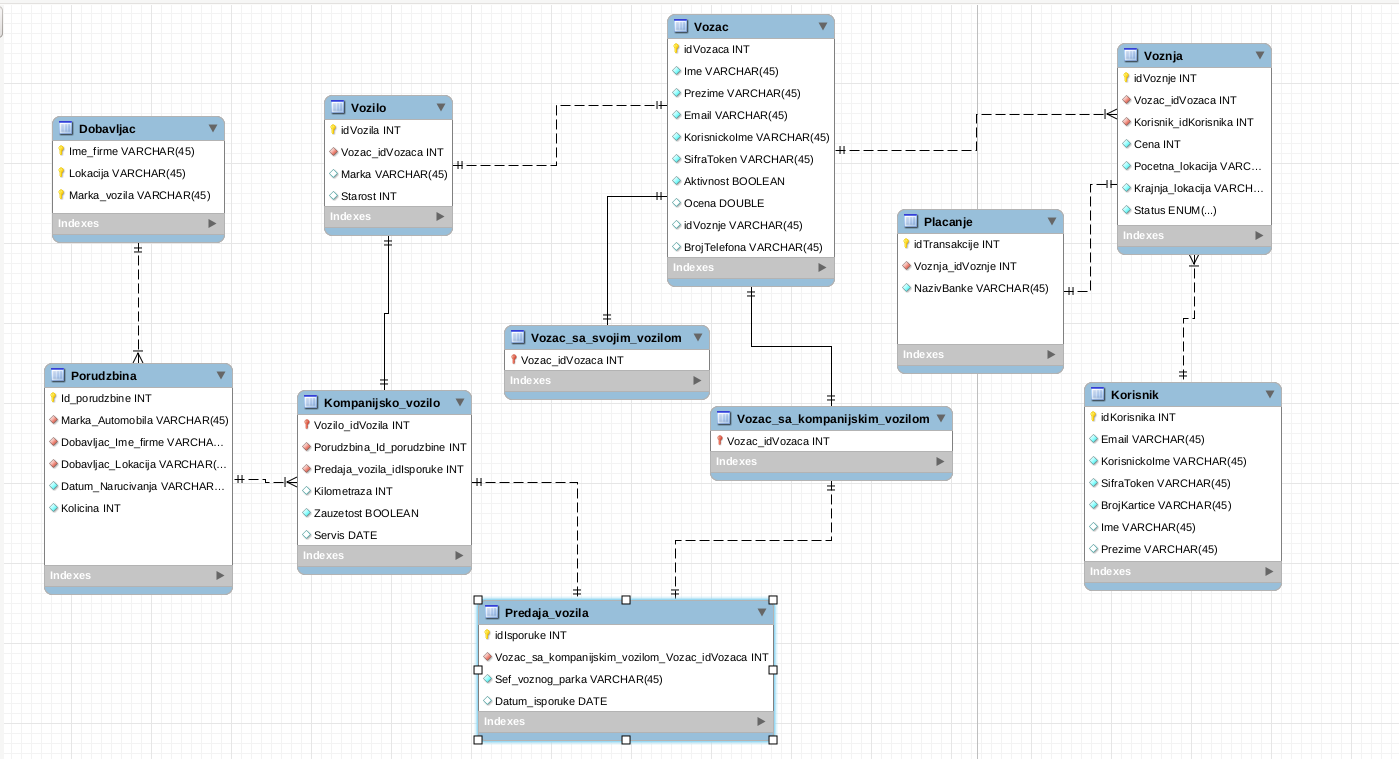
\includegraphics[width=\textwidth]{Slike/EERDijagramBazePodataka.png}
\end{center}
    \caption{Šema baze podataka}
\label{fig:bazaPodataka}
\end{figure}

\subsection{\textbf{Nezavisni entiteti}}Nezavisni entiteti su:
    \begin{itemize}
        \item Vozač
        \item Korisnik
        \item Vozilo
        \item Dobavljač
    \end{itemize}

\begin{flushleft}
\underline{Vozač}
\end{flushleft}
Svaki vozač ima email i šifru pomoću kojih pristupa svom nalogu. Vozač postaje aktivan kad se prijavi. Atributi:
\begin{itemize}
    \item Ime
    \item Prezime
    \item korisnickoIme - korisničko ime vozača pomoću kojeg se prijavljuje
    \item Ocena - ocena koju je dobio od korisnika u određenoj vožnji
    \item Email - email sa kojim se vozač registrovao
    \item SifraToken - enkriptovana sifra vozača
    \item Aktivnost - trenutno stanje vozača, može biti aktivan ili neaktivan
    \item IdVoznje - vožnje u kojima je vozač učestvovao
    \item BrojTelefona
\end{itemize}

\begin{flushleft}
\underline{Korisnik}
\end{flushleft}
Kao i vozač, i korisnik ima svoj nalog. Korisnik se prijavljuje kad mu je potrebna vožnja. Za registraciju mora koristiti email. Atributi:
\begin{itemize}
    \item Ime
    \item Prezime
    \item KorisnickoIme - korisničko ime pomoću kojeg se korisnik prijavljuje
    \item Email - email korisnika pomoću kojeg se registruje
    \item SifraToken - enkriptovana šifra korisnika
    \item BrojKartice - broj kartice pomoću koje korisnik vrši plaćanje
\end{itemize}

\begin{flushleft}
\underline{Vozilo}
\end{flushleft}
Sadrži informacije o vozilima svih vozača. Atributi:
\begin{itemize}
    \item Vozac\_idVozaca - Id vozača koji koristi to vozilo
    \item Marka
    \item Starost
\end{itemize}

\begin{flushleft}
\underline{Dobavljač}
\end{flushleft}
Sadrži informacije o dobavljačima od kojih nabavljamo vozila. Atributi:
\begin{itemize}
    \item Ime\_firme
    \item Lokacija
    \item Marka\_vozila
\end{itemize}


\subsection{\textbf{Izvedeni entiteti}}
Izvedeni entiteti su:
\begin{itemize}
    \item Vozač sa svojim vozilom
    \item Vozač sa kompanijskim vozilom
    \item Kompanijsko vozilo
\end{itemize}

\begin{flushleft}
\underline{Vozač sa svojim vozilom}
\end{flushleft}
Predstavlja specijalizaciju eniteta vozač. Sadrži informacije o vozačima koji imaju sopstveno vozilo. Atributi:
\begin{itemize}
    \item Vozac\_idVozaca - Id vozača koji ima sopstveno vozilo, strani ključ ka entitetu vozač
\end{itemize}

\begin{flushleft}
\underline{Vozač sa kompanijskim vozilom}
\end{flushleft}
Predstavlja specijalizaciju entiteta vozač. Sadrži informacije o vozačima koji nemaju sopstveno vozilo. Atributi:
\begin{itemize}
    \item Vozac\_idVozaca - Id vozača koji nema sopstveno vozilo, strani ključ ka entitetu vozač
\end{itemize}

\begin{flushleft}
\underline{Kompanijsko vozilo}
\end{flushleft}
Predstavlja specijalizaciju entiteta vozilo. Sadrži informacije o vozilima koji su u vlasnistvu firme i izdaju se vozačima na korišćenje. Atributi:
\begin{itemize}
    \item Vozilo\_idVozila - strani ključ ka entitetu vozilo.
    \item Porudzbina\_id\_porudzbine - redni broj porudžbine u kojoj je vozilo naručenoču.
    \item Predaja\_vozila\_idisporuke - strani ključ na tabelu predaja vozila
    \item Zauzetost - indikator da li je vozilo predato nekom vozaču ili ne
    \item Kilometraza
    \item Servis
\end{itemize}


\subsection{\textbf{Agregirani entiteti}}
Agregirani entiteti su:
\begin{itemize}
    \item Vožnja
    \item Plaćanje
    \item Predaja vozila
    \item Porudžbina
\end{itemize}

\begin{flushleft}
\underline{Vožnja}
\end{flushleft}
Sadrži informacije o svim vožnjama. Atributi:
\begin{itemize}
    \item Vozac\_idVozaca - id vozača koji vozi korisnika ka željenoj lokaciji, strani ključ ka entitetu Vozač.
    \item Vozac\_idKorisnika - id korisnika koji je traži prevoz, strani ključ ka entitetu Korisnik.
    \item Cena - naknada koju korisnik treba da plati za izvršenu uslugu.
    \item Pocetna\_lokacija - lokacija sa koje je korisnik zatrašio uslugu.
    \item Krajnja\_lokacija - lokacija na koju korisnik želi da se preveze.
    \item Status - trenutni status vožnje.
\end{itemize}

\begin{flushleft}
\underline{Plaćanje}
\end{flushleft}
Sadrži informacije o platnim transakcijama za svaku vožnju. Atributi:
\begin{itemize}
    \item Voznja\_idVoznje - id vožnje za koju se vrši plaćanje.
    \item NazivBanke - Naziv banke koja vrši transakciju.
\end{itemize}

\begin{flushleft}
\underline{Predaja vozila}
\end{flushleft}
Sadrži informacije o predatim vozilima vozačima koji nemaju svoja. Atributi:
\begin{itemize}
    \item Vozac\_sa\_kompanijskim\_vozilom\_Vozac\_idVozaca - strani ključ na entitet Vozač sa kompanijskim vozilom.
    \item Sef\_voznog\_parka - ime osobe koja vrši dobavljanje vozila.
    \item Datum
\end{itemize}

\begin{flushleft}
\underline{Porudžbina}
\end{flushleft}
Sadrži informacije o naručenim vozilima vozačima koji nemaju svoja. Atributi:
\begin{itemize}
    \item Marka\_automobila - strani ključ na entitet Dobavljač, sadrži informacije o marki automobila koji se naručuje.
    \item Dobavljac\_ime\_firme - strani ključ na entitet Dobavljač, sadrži informacije o nazivu firme od koje naručujemo vozila.
    \item Dobavljac\_Lokacija - strani ključ na entitet Dobavljač, sadrži informacije o lokaciji firme od koje naručujemo vozila.
    \item Datum\_narucivanja
    \item Kolicina - broj vozila koji se naručuje.
\end{itemize}
